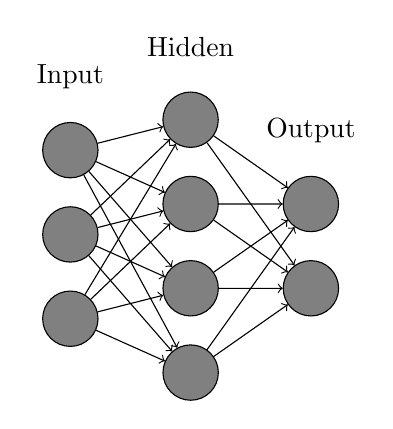
\begin{tikzpicture}[
    scale=1.2,
    basic/.style={draw,fill=gray,text badly centered,minimum width=2em},
    circ/.style={basic,circle,minimum width=2em},
]
    %inputs
    \node[circ] (i1) {};
    \node[circ,below of=i1,yshift=-0.2em] (i2) {};
    \node[circ,below of=i2,yshift=-0.2em] (i3) {};
    \node[above of=i1,yshift=-0.2em] {Input};

    \node[circ,right of=i1,xshift=1.5em,yshift=1.1em] (h1) {};
    \node[circ,below of=h1,yshift=-0.2em] (h2) {};
    \node[circ,below of=h2,yshift=-0.2em] (h3) {};
    \node[circ,below of=h3,yshift=-0.2em] (h4) {};
    \node[above of=h1,yshift=-0.2em] {Hidden};

    \node[circ,right of=h2,xshift=1.5em] (o1) {};
    \node[circ,right of=h3,xshift=1.5em] (o2) {};
    \node[above of=o1,yshift=-0.2em] {Output};

    \draw[->] (i1) -- (h1);
    \draw[->] (i1) -- (h2);
    \draw[->] (i1) -- (h3);
    \draw[->] (i1) -- (h4);
    \draw[->] (i2) -- (h1);
    \draw[->] (i2) -- (h2);
    \draw[->] (i2) -- (h3);
    \draw[->] (i2) -- (h4);
    \draw[->] (i3) -- (h1);
    \draw[->] (i3) -- (h2);
    \draw[->] (i3) -- (h3);
    \draw[->] (i3) -- (h4);

    \draw[->] (h1) -- (o1);
    \draw[->] (h1) -- (o2);
    \draw[->] (h2) -- (o1);
    \draw[->] (h2) -- (o2);
    \draw[->] (h3) -- (o1);
    \draw[->] (h3) -- (o2);
    \draw[->] (h4) -- (o1);
    \draw[->] (h4) -- (o2);
\end{tikzpicture}